\documentclass[10.5pt,compsoc,UTF8]{CjC}
\usepackage{CTEX}
\usepackage{graphicx}
\usepackage{footmisc}
\usepackage{subfigure}
\usepackage{url}
\usepackage{multirow}
\usepackage{multicol}
\usepackage[noadjust]{cite}
\usepackage{amsmath,amsthm}
\usepackage{amssymb,amsfonts}
\usepackage{booktabs}
\usepackage{color}
\usepackage{ccaption}
\usepackage{booktabs}
\usepackage{float}
\usepackage{fancyhdr}
\usepackage{caption}
\usepackage{xcolor,stfloats}
\usepackage{comment}
\usepackage[colorlinks=true, linkcolor=blue, citecolor=blue, urlcolor=blue]{hyperref}
\usepackage{cleveref}
\setcounter{page}{1}
% \graphicspath{{figures/}}
\usepackage{cuted}
\usepackage{captionhack}
\usepackage{epstopdf}
\usepackage{gbt7714}
\usepackage{stfloats}
\usepackage{amsmath}
\usepackage{arydshln}
%===============================%

%=======设置奇偶页页眉=======%
\headevenname{\mbox{\quad} \hfill  \mbox{\zihao{-5}{计\quad \quad 算\quad \quad 机\quad \quad 学\quad \quad 报} \hspace {50mm} \mbox{2023 年}}}%
\headoddname{? 期 \hfill
作者姓名等:论文题目}
%=======设置奇偶页页眉=======%

\renewcommand{\thefootnote}{\fnsymbol{footnote}}
\setcounter{footnote}{0}
\renewcommand\footnotelayout{\zihao{5-}}
\newtheoremstyle{mystyle}{0pt}{0pt}{\normalfont}{1em}{\bf}{}{1em}{}
\theoremstyle{mystyle}
\renewcommand\figurename{figure~}
\renewcommand{\thesubfigure}{(\alph{subfigure})}
\newcommand{\upcite}[1]{\textsuperscript{~\cite{#1}}}
\renewcommand{\labelenumi}{(\arabic{enumi})}
\newcommand{\tabincell}[2]{\begin{tabular}{@{}#1@{}}#2\end{tabular}}
\newcommand{\abc}{\color{white}\vrule width 2pt}
\renewcommand{\bibsection}{}
\makeatletter
\renewcommand{\@biblabel}[1]{[#1]\hfill}
\makeatother
\setlength\parindent{2em}

\pagestyle{CjCheadings}
\setmainfont{Times New Roman}

%===========================================================%
\begin{document}

\hyphenpenalty=50000
\makeatletter
\newcommand\mysmall{\@setfontsize\mysmall{7}{9.5}}
\newenvironment{tablehere}
  {\def\@captype{table}}

\let\temp\footnote
\renewcommand \footnote[1]{\temp{\zihao{-5}#1}}

%=======设置首页页眉=======%
\thispagestyle{empty}%
\begin{table*}[!t]
\vspace {-13mm}
\onecolumn
\noindent\begin{tabular}{p{168mm}}
\zihao{5-}
第??卷\quad 第?期 \hfill 计\quad 算\quad 机\quad 学\quad 报\hfill Vol. ??  No. ?\\
\zihao{5-}
20??年?月 \hfill CHINESE JOURNAL OF COMPUTERS \hfill ???. 20??\\
\hline\\[-5.5mm]
\hline\end{tabular}\end{table*}
%=======设置首页页眉=======%

%中文标题、作者与注脚
{
\centering
\vspace {11mm}
{\zihao{2} \heiti 基于大语言模型, 法律引导的的案例融合方法, 用于司法判决预测 }

\vskip 5mm

{\zihao{3}\fangsong 张丁文$^{1}$ \quad  梁正涛$^{1}$  \quad 朱伊丽$^{1}$ \quad  秦永彬$^{1}$ \quad  陈艳平$^{1}$ \quad 黄瑞章$^{1}$}
\footnote{\noindent \zihao{6}\songti 收稿日期:\quad \quad -\quad -\quad ;
%基金
}

\vspace {1mm}

\zihao{6}{$^{1)}$贵州大学 计算机科学与技术与技术学院 贵阳  550004}



}%中文标题、作者与注脚

\vskip 5mm

\zihao{5-}{
\setlength{\baselineskip}{16pt}\selectfont{
\noindent {\heiti 摘\quad 要\quad }
法律判决预测(LJP)是推动司法智能化的关键研究领域。然而,现有方法普遍面临挑战:传统模型因其“黑箱”特性和对复杂法律逻辑处理能力的不足而受到诟病;而直接应用大型语言模型(LLMs)则面临内容“幻觉”、缺乏专业法律知识等固有缺陷。为应对这些挑战,本文提出一种法律指导的类案融合判决方法。该方法将LJP任务分解为多个逻辑子任务:首先,利用LLM提取判决的核心要素;其次,通过检索增强生成(RAG)机制,并行地从法律条文库和历史案例库中获取法律规范与相似判例;最后,将多源信息输入LLM进行综合推理,生成结构化判决。
本研究旨在通过为LLM提供明确的法律依据和司法实践参考,系统性地提升判决质量。实验结果表明,该方法在罪名和刑期预测任务上的F1分数分别达到了0.7743和0.5525。相较于同样结合了外部知识库的先进基准模型,F1分数分别提升了2.46和8.34个百分点。尤其在对司法实践经验有高度依赖的刑期预测上,性能提升显著。这证明了本方法通过有效融合多源异构知识,能够显著增强判决预测的准确性与可解释性,为构建更可靠、更透明的智能司法判决系统提供了新的解决方案。
}}

\vspace {5mm}

\zihao{5-}{\noindent
{\heiti 关键词 \quad }{大语言模型;检索增强生成;判决预测;智慧法院;}
}\par\noindent
\zihao{5-}{\heiti 中图法分类号\quad } TP\rm{\quad \quad \quad     }
{\heiti DOI号:\quad } *投稿时不提供DOI号

\vskip 5mm


\begin{center}
\zihao{3}{ \heiti Laws-Guided Precedent Case Fusion based-on LLM for Legal Prediction}\\
\vspace {5mm}
\zihao{5}{ Dingwen Zhang$^{1)}$ Zhentao liang$^{1)}$ Yili Zhu$^{1)}$ Yongben Qin$^{1)}$ Yanpin Chen$^{1)}$ Ruizhang Huang$^{1)}$}\\
\vspace {1mm}
\zihao{6}{{$^{1)}$Department of Computer and Science, Guizhou University, Guiyang 550004}}


\end{center}

\zihao{5}{
{\noindent\bf Abstract}\quad
%英文摘要
\zihao{5}{\noindent Legal Judgment Prediction (LJP) is a critical research area for advancing judicial intelligence. However, existing methods face significant challenges. Traditional models are often criticized for their "black-box" nature and inability to handle complex legal logic, while the direct application of Large Language Models (LLMs) is plagued by inherent flaws such as content "hallucinations" and a lack of domain-specific legal knowledge. To address these issues, this paper proposes a law-guided case fusion judgment method. This approach decomposes the LJP task into several logical sub-tasks: first, it leverages an LLM to extract core adjudicative elements; second, it employs a Retrieval-Augmented Generation (RAG) mechanism to concurrently retrieve authoritative legal statutes and highly similar precedents; finally, it inputs this multi-source information into an LLM for comprehensive reasoning to generate a structured judgment.
This research aims to systematically improve prediction quality by providing the LLM with explicit legal grounding and practical judicial references. Experimental results demonstrate that our method achieves F1-scores of 0.7743 and 0.5525 on charge and sentencing prediction tasks, respectively. Compared to an advanced baseline model that also utilizes RAG, our approach shows improvements of 2.46 and 8.34 percentage points. The performance gain is particularly significant in sentencing prediction, a task that heavily relies on judicial practice. This validates that our method, by effectively fusing multi-source heterogeneous knowledge, can significantly enhance the accuracy and interpretability of LJP, offering a novel solution for building more reliable and transparent intelligent judicial systems.
\par}}

\vspace {5mm}

\zihao{5-}{\noindent
{\heiti Key words \quad }{Large Language Models; Retrieval-Augmention Generation; Judgment Prediction; Smart Courts;}
}\par\noindent

\zihao{5}
\vskip 1mm

\begin{multicols}{1}
\section{\heiti 引言}

随着信息技术飞速发展,“数字法院”建设已成为全球司法现代化的重要趋势。这使得对智能化司法审判解决方案的需求日益迫切,尤其是在刑事案件审判领域。该领域的核心目标是提升司法判决的准确性、一致性和效率~\cite{aletras2016predicting}。在此背景下,法律判决预测(LJP)作为法律人工智能领域的基础性、关键性研究任务,受到学术界和实务界的广泛关注。LJP通过分析案件事实描述,自动预测法院判决结果,辅助法官及其他法律从业者提升案件处理效率。

LJP技术的早期研究主要依赖人工构建的规则系统和传统统计机器学习方法\cite{katz2017general,keown1980mathematical},例如支持向量机(SVM)\cite{boella2011using,kim2015legal}。Sulea等人~\cite{sulea2017exploring}构建了一种结合多个SVM分类器输出平均概率的集成系统。该模型以案情事实描述和时间跨度信息为输入,能够输出判决结果、法律范围和估算判决日期等信息。Katz等人~\cite{katz2017general}使用随机森林,从案情描述中提取有效特征,预测美国最高法院的判决结果。然而,这些方法未能有效挖掘深层文本特征。由于其人工设计的特性,这些方法需要大量人力成本,难以广泛应用于其他领域。
\begin{figure*}[htbp]
	\centering
	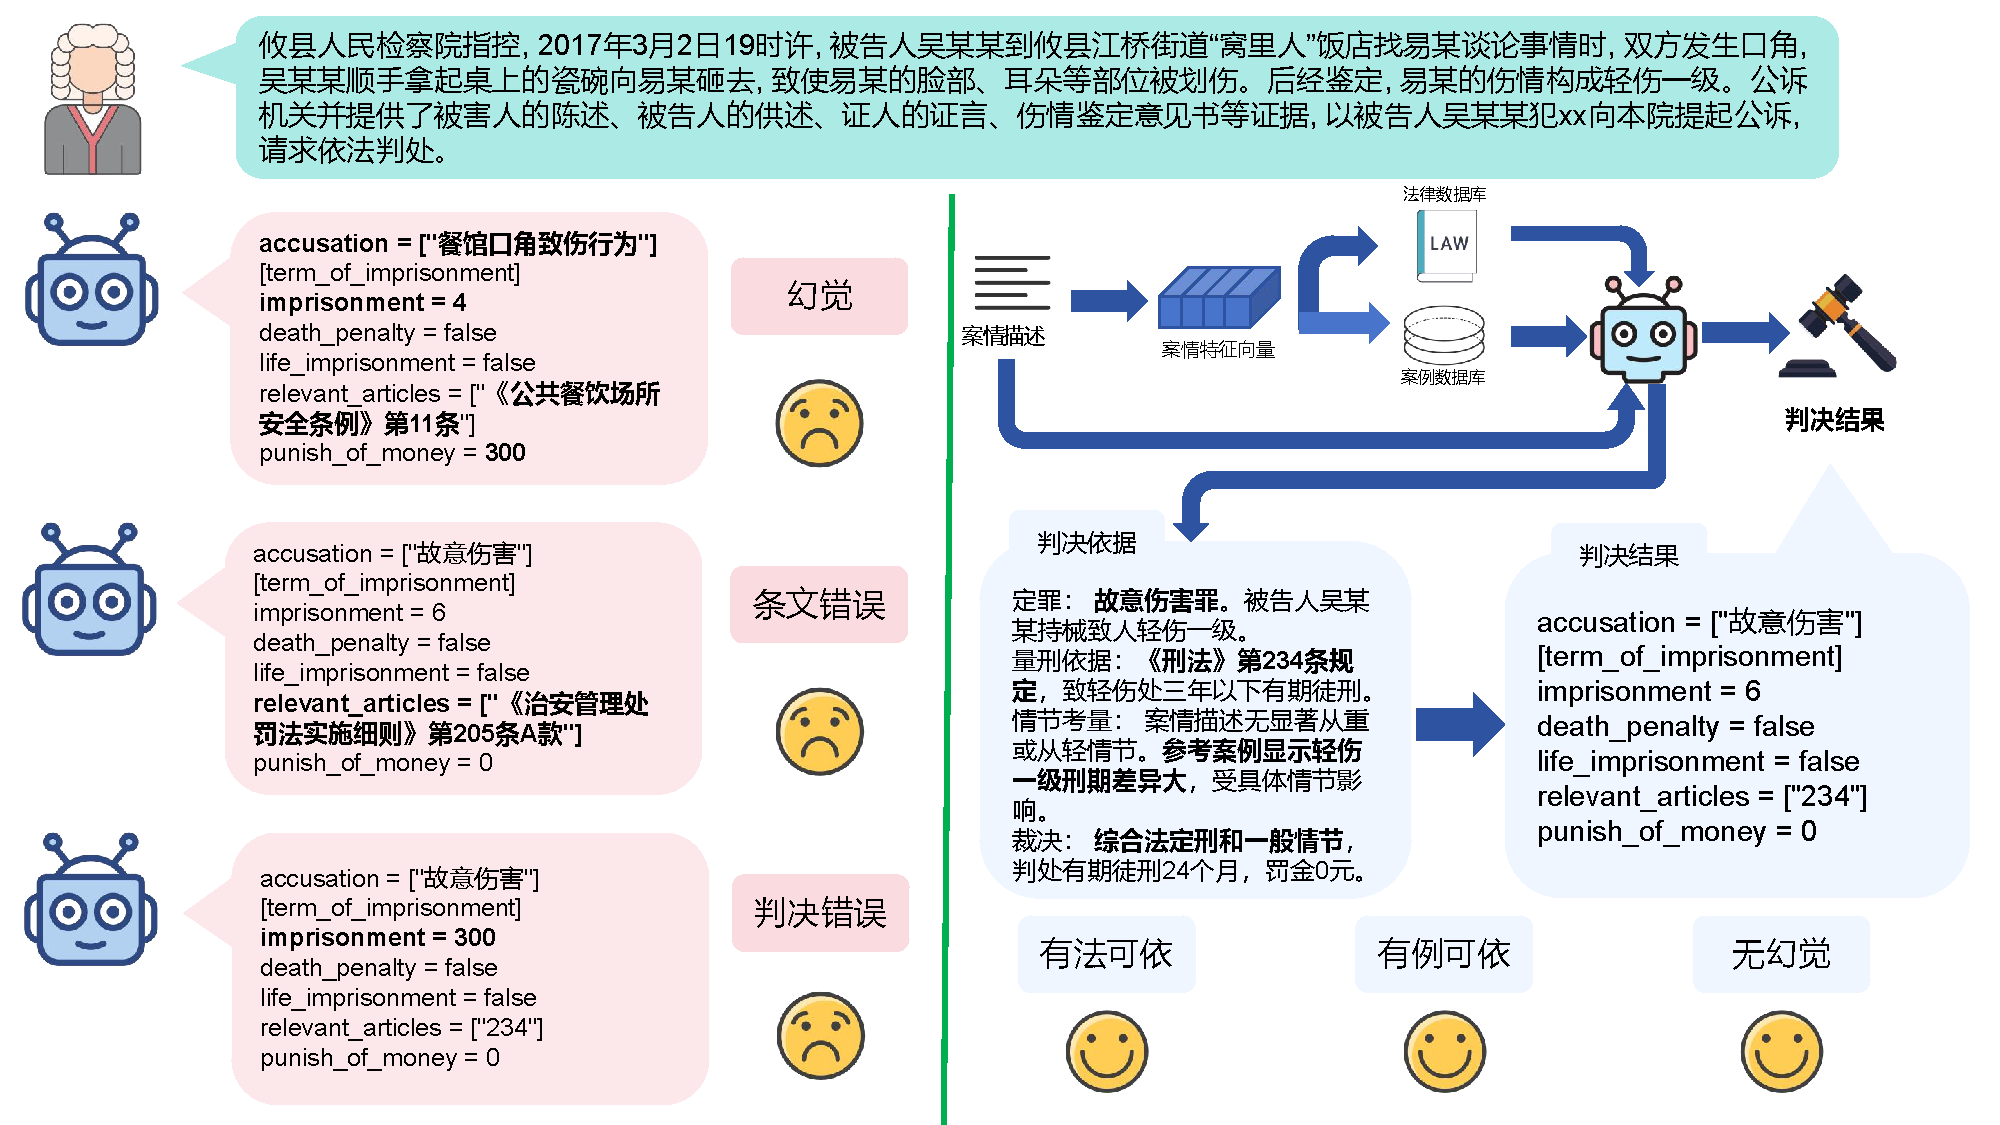
\includegraphics[width=1\textwidth]{fig/motivation.pdf}
	\caption{基于法条约束与类案融合的可解释司法判决预测动机}
	\label{fig:motivation}
\end{figure*}
此外,许多早期深度学习LJP模型如同“黑箱”般运作,其决策过程缺乏透明度和可解释性。模型的不可解释性构成了其在司法实践中推广应用的主要障碍\cite{ling2017program,ma2021law,nye2021show}。法官难以干预模型的审判逻辑或理解其预测依据,从而削弱了模型的实用价值。缺乏可解释性还可能引发伦理问题,尤其当模型从历史数据中学习到潜在偏见时,可能导致不公正或不一致的判决结果~\cite{luo2017learning,lv2022improving}。

尽管大型语言模型(LLM)因其卓越的语言理解能力而备受期待~\cite{jiang2023legal},但在法律领域的直接应用暴露出若干固有缺陷。一个核心问题是LLM倾向于产生“幻觉”(Hallucinations),即生成与客观事实或用户输入不符的内容~\cite{lewis2020retrieval,zheng2021when}。在法律语境下,这可能表现为援引虚假判例、引言或内部引证,从而导致判决不公,甚至判决错误。研究表明,在处理特定法律查询时,LLM的幻觉率可能高达69\%至88\%~\cite{Dahl_2024}。这种现象通常源于模型在缺乏可验证法律依据的情况下,尝试进行推理或生成信息~\cite{zhong2020iteratively,zhong2020jec-qa}。

针对传统方法在可解释性和处理复杂法律逻辑方面的不足,以及通用LLM在直接应用中面临的幻觉、法律知识基础缺乏和专业推理能力弱等问题,本研究提出了一种基于法条约束与类案融合的可解释司法判决预测方法。该方法通过提取判决核心要素(即犯罪核心要素与证据核心要素),旨在减少判决过程中的干扰因素,提供准确且核心的信息。
此外,本研究还引入相似案例,旨在为LLM提供司法实践层面的参考,使其理解法律条文在具体情境下的应用方式,并学习裁判经验。最后,LLM作为核心推理引擎,对这些多源异构信息进行综合分析和推理。它综合考量法律原则、司法解释及类案判例的指导作用,输出结构化的判决结果。本研究的方法无需对整个大型语言模型进行重新训练,它将复杂的LJP任务分解为多个子任务,使得整个推理过程更为透明和模块化。与一些端到端的“黑箱”模型相比,这种设计不仅有助于提升整体预测的鲁棒性,还为理解和调试模型行为提供了便利。

\section{\heiti 相关工作}
在数据和算力受限的背景下,LJP的早期探索主要依赖统计学方法。
例如,Kort~\cite{kort1957predicting} 通过多因素复合分析,揭示了美国最高法院处理特定案件时的判决规律。
该时期的研究还包括应用专家系统将法律知识转化为计算机可处理的规则~\cite{susskind1986expert}。
然而,这些传统方法的核心局限在于它们对噪声数据的高度敏感性以及对人工规则的过度依赖。
法律文本的复杂性和模糊性使得规则制定和特征标注异常困难。
简单的数学模型难以捕捉司法实践中复杂多样的非线性影响因素,从而限制了其预测性能和泛化能力~\cite{deng2023syllogistic,dong2021legal}。


为解决此问题,研究转向了机器学习和文本挖掘技术~\cite{chen2013text,goncalves2005evaluating}。
学者们通过将案件事实作为输入、判决结果作为标签,利用支持向量机(SVM)~\cite{kianmehr2006crime} 或随机森林(Random Forest)~\cite{sulea2017exploring}等模型,从案情描述中自动学习特征以预测判决。
例如,Katz等~\cite{sulea2017exploring} 应用随机森林模型,有效提取了影响美国最高法院判决的关键特征。
这类方法的优势在于增强了模型对非线性关系的建模能力,并初步实现了特征提取的自动化。
然而,其短板也十分明显:模型性能高度依赖于人工设计的特征工程,这不仅耗费大量人力,而且难以挖掘文本背后深层次的语义信息,导致其难以迁移至更广泛的法律场景。


随着深度学习的兴起,LJP研究迎来了新的突破。
基于深度神经网络的模型能够自动捕捉文本中更复杂、更抽象的特征~\cite{cheng2025legal,feng2022legal,jiang2018interpretable,wang2019hierarchical}。
Luo等~\cite{huang2019improved} 提出的模型利用注意力机制,动态识别并聚焦于事实描述中最关键的部分,有效关联了案件事实与罪名认定,显著提升了预测准确性。
为了更全面地模拟司法过程,Yue等~\cite{yue2021neurjudge} 构建了一个情境感知的多任务学习框架(NeurJudge),它通过协同法条预测、罪名预测等多个子任务,使模型学习到任务间的共享信息,从而提升了主任务的性能。
受BERT等模型成功的启发,法律AI领域涌现出Legal-BERT~\cite{liu2021robustly,chalkidis2020legal,deepa2021bidirectional,devlin2019bert,fan2022multi}、Lawformer~\cite{xiao2021lawformer,du2022glm,fei2023lawbench,oana-maria2018e-snli}等在海量法律语料上预训练的模型。
它们通过迁移学习,将从大规模无标注文本中学到的丰富语言知识应用于下游任务,相较于传统机器学习模型,获得了显著的性能提升~\cite{cui2021pre,houlsby2019parameter,hu2018few,zhang2023contrastive}。
尽管深度学习极大地推动了LJP的发展,但深度学习模型如同“黑箱”般运作,其决策过程缺乏透明度和可解释性。尤其当数据存在潜在偏见时,深度学习模型可能直接导致不公正或不一致的判决结果。


\begin{figure*}[htpb]
	\centering
	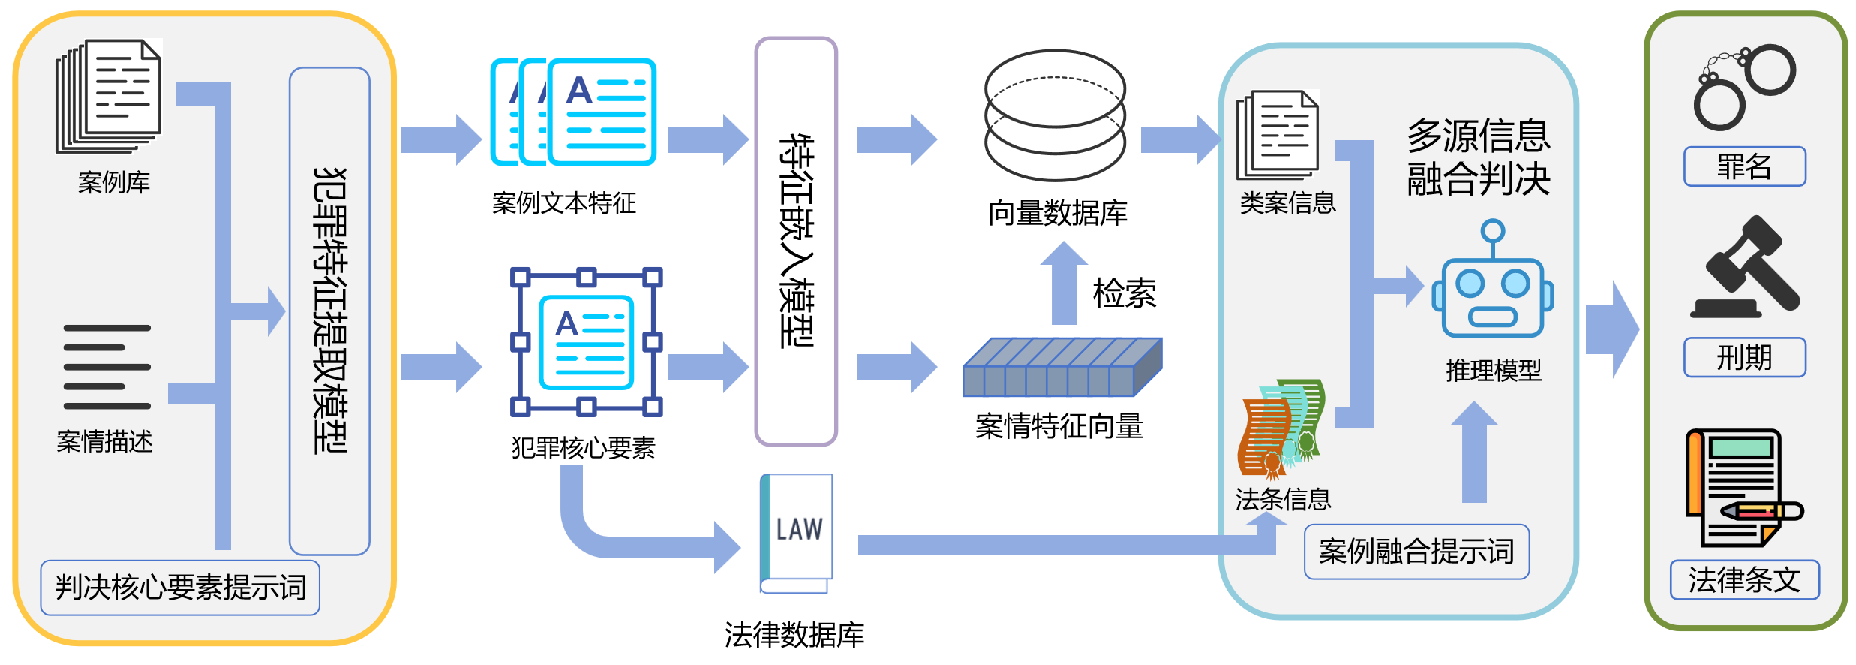
\includegraphics[width=1\textwidth]{fig/method2.pdf}
	\caption{基于法条约束与类案融合的可解释司法判决预测方法}
	\label{fig:main}
\end{figure*}

LLM因其强大的复杂上下文推理能力、庞大的预训练知识库和良好的可解释性,被期望成为下一代LJP的新范式~\cite{wu2020de-biased,yang2023baichuan,yao2020refining}。
当前,以LLM为核心的技术范式已成为研究热点。其强大的常识推理和零样本/少样本学习能力为LJP带来了新的可能性~\cite{brown2020language,huang2022towards,shu2024large,wen2024review}。
将LLM直接应用于严肃的法律领域仍面临严峻挑战。
未经充分优化的通用LLM在处理法律问题时,容易出现“幻觉”(Hallucination)~\cite{cui2023survey,radford2025improving,raffel2020exploring}。这可能表现为捏造不存在的法律条文、引用错误的案例,或给出超出法定范围的量刑建议~\cite{lewis2020retrieval}。
为解决LLM的幻觉问题,主要优化思路分为两条路径。一是通过提示工程(Prompt Engineering)引导模型,例如利用“思维链”(Chain of Thought)~\cite{kojima2022large,izacard2021leveraging,rajani2019explain,talmor2019leap,wang2023self,wei2022chain}或司法三段论~\cite{huang2023lawyer,trautmann2022legal,xu2023superclue,yu2022legal}来规范其推理逻辑。
然而,为特定任务精心设计的提示词(Prompt)往往缺乏通用性,难以直接迁移至其他法律任务,这限制了其可扩展性;
二是以法律专业数据对LLM进行微调,例如Lawyer LLaMA~\cite{chen2020recall,yue2021circumstances},使其具备更强的“法律素养”。
尽管微调是提升专业性的有效途径~\cite{hu2021lora,hu2022lora,zelikman2024star},但LLM微调存在以下问题:首先,微调的成功依赖于高质量标注数据和大量计算资源。
其次,微调后的LLM知识体系是静态的,其知识停留在训练数据集的时间点,无法实时跟进法律法规的更新和司法解释的演进~\cite{li2021prefix,zhang2024comprehensive}。
最后,微调过程还可能导致模型对其通用知识的“灾难性遗忘”~\cite{chen2020recall},损害其基础推理能力。
因此,本研究提出一种基于LLM并由法律引导的案例融合方法。
该方法将提示词工程与检索增强技术相结合,以实现司法智能审判的可信判决。
该方法通过特定的提示词提取案例描述的关键判决核心要素,从而保留司法审判理论的核心要素并去除冗余噪声。
此外,通过引入案例数据库和法律条文数据库,为LLM提供精确的罪名定义和司法实践案例,以综合理论知识与实践经验。
最后,利用多源异构信息进行综合分析与推理,做出最终的司法判决。
该方法无需微调LLM,并且可以通过引入新的法律条文和案例,提供最新的法理知识,从而避免LLM因缺少相关知识而产生幻觉。



\section{\heiti 方法}
\subsection{\heiti 总体流程}
\begin{multicols}{1}
	\begin{figure}[H]
		\centering
		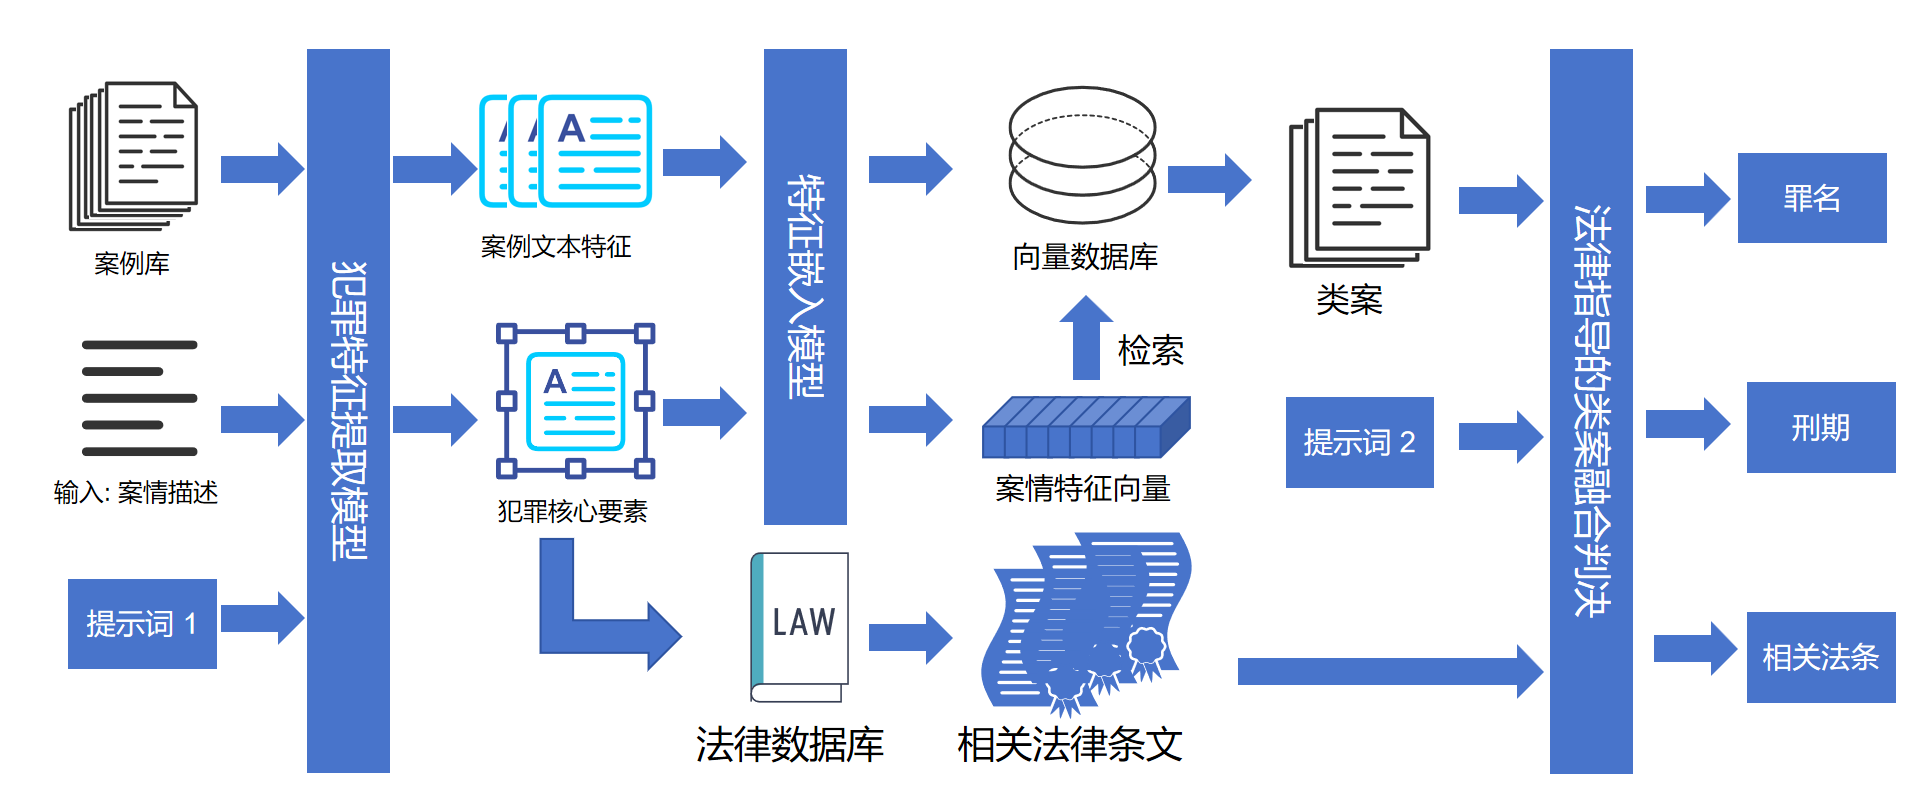
\includegraphics[width=1\textwidth]{fig/main.png}
		\caption{基于大语言模型, 法律引导的的案例融合方法, 用于司法判决预测流程}
		\label{fig:main}
	\end{figure}
\end{multicols}
本位提出的司法判决预测方法,其核心在于构建一个能够有效整合案件事实、法律法规及类案判例的智能推理框架。整体流程如图\ref{fig:main}所示。
首先,系统接收待判决案件的详细事实描述($C$),并利用预训练的大语言模型进行初步语义分析和关键信息抽取。该模型通过自然语言理解能力,从复杂的案情描述中识别并初步推断出罪名类别、犯罪构成要件(包括主体、主观、客体、客观)及证据特征等核心法律要素,形成结构化的犯罪特征表示($F$)。
其次,基于抽取的犯罪特征$F$,系统并行地从两个专门构建的法律知识库中检索相关信息。一方面,从权威的法律条文数据库中检索出与案件特征$F$高度相关的法律法规条款集合($L$)。另一方面,从海量的历史案例数据库中智能检索出与当前案件在罪名构成、事实情节和证据方面最为相似的判例集合($S$)。
最后,将原始案件事实描述$C$、检索到的相关法律条文$L$以及相似判例$S$共同作为上下文信息,输入至大语言模型,输出胡最终的判决结果。该模型作为核心推理引擎,通过整合这些多源异构信息,综合考量法律原则、司法解释及类案判例的指导作用,有效弥补了LLM在法律专业知识和复杂逻辑推理方面的固有局限性,显著增强了判决预测的专业性、准确性和可解释性。
\section{\heiti 实验}

\subsection{\heiti 实验数据}
\begin{table*}[htbp]
	\centering
	\caption{ 法律判决预测结果的对比}
	\begin{tabular}{lcccccc}
		\toprule
		\textbf{模型} & \multicolumn{3}{c}{\textbf{罪名}} & \multicolumn{3}{c}{\textbf{刑期}}                                                               \\
		\cmidrule(lr){2-4} \cmidrule(lr){5-7}
		            & \textbf{精确率}                    & \textbf{召回率}                    & \textbf{F1分数} & \textbf{精确率} & \textbf{召回率} & \textbf{F1分数} \\
		\midrule
		MTL-Fusion  & 0.6861                          & 0.6911                          & 0.6886        & 0.3512       & 0.3567       & 0.3539        \\
		Lawformer   & 0.6927                          & 0.7082                          & 0.7004        & 0.3581       & 0.3629       & 0.3605        \\
		BERT        & 0.7011                          & 0.7178                          & 0.7094        & 0.4311       & 0.4308       & 0.4309        \\
		LawChatGLM  & 0.7517                          & 0.7478                          & 0.7497        & 0.4712       & 0.4671       & 0.4691        \\
		Ours        & \textbf{0.7797}                          & \textbf{0.7689}                          & \textbf{0.7743}        & \textbf{0.5578}       & \textbf{0.566}        & \textbf{0.5525}        \\
		\bottomrule
	\end{tabular}
	\label{tab:performance_comparison}
\end{table*}

实验使用开源的数据集CAIL 2018~\cite{xiao2018cail2018largescalelegaldataset},共涵盖1927685个案例,覆盖202种刑事罪名和183条刑法法规,其中训练集有1927685条数据,测试集有216829条数据;在数据集中,多被告案件法条分布往往存在长尾分布现象。如图\ref{fig:acc_dis}所示,各个法条在判决结果中的出现频率及其占比有较大的不同。在测试数据的法条分布中,占比最高的5个罪行是,盗窃,危险驾驶,故意伤害和交通肇事,其占比分别达到了20.63\%,17.17\%,10.49\%,8.29\%,7.33\%;占比最高的10种罪行占总测试数据的73.58\%。而占比最少的100种罪行只占到总数据的1.83\%。
\begin{figure}[H]
		\centering
		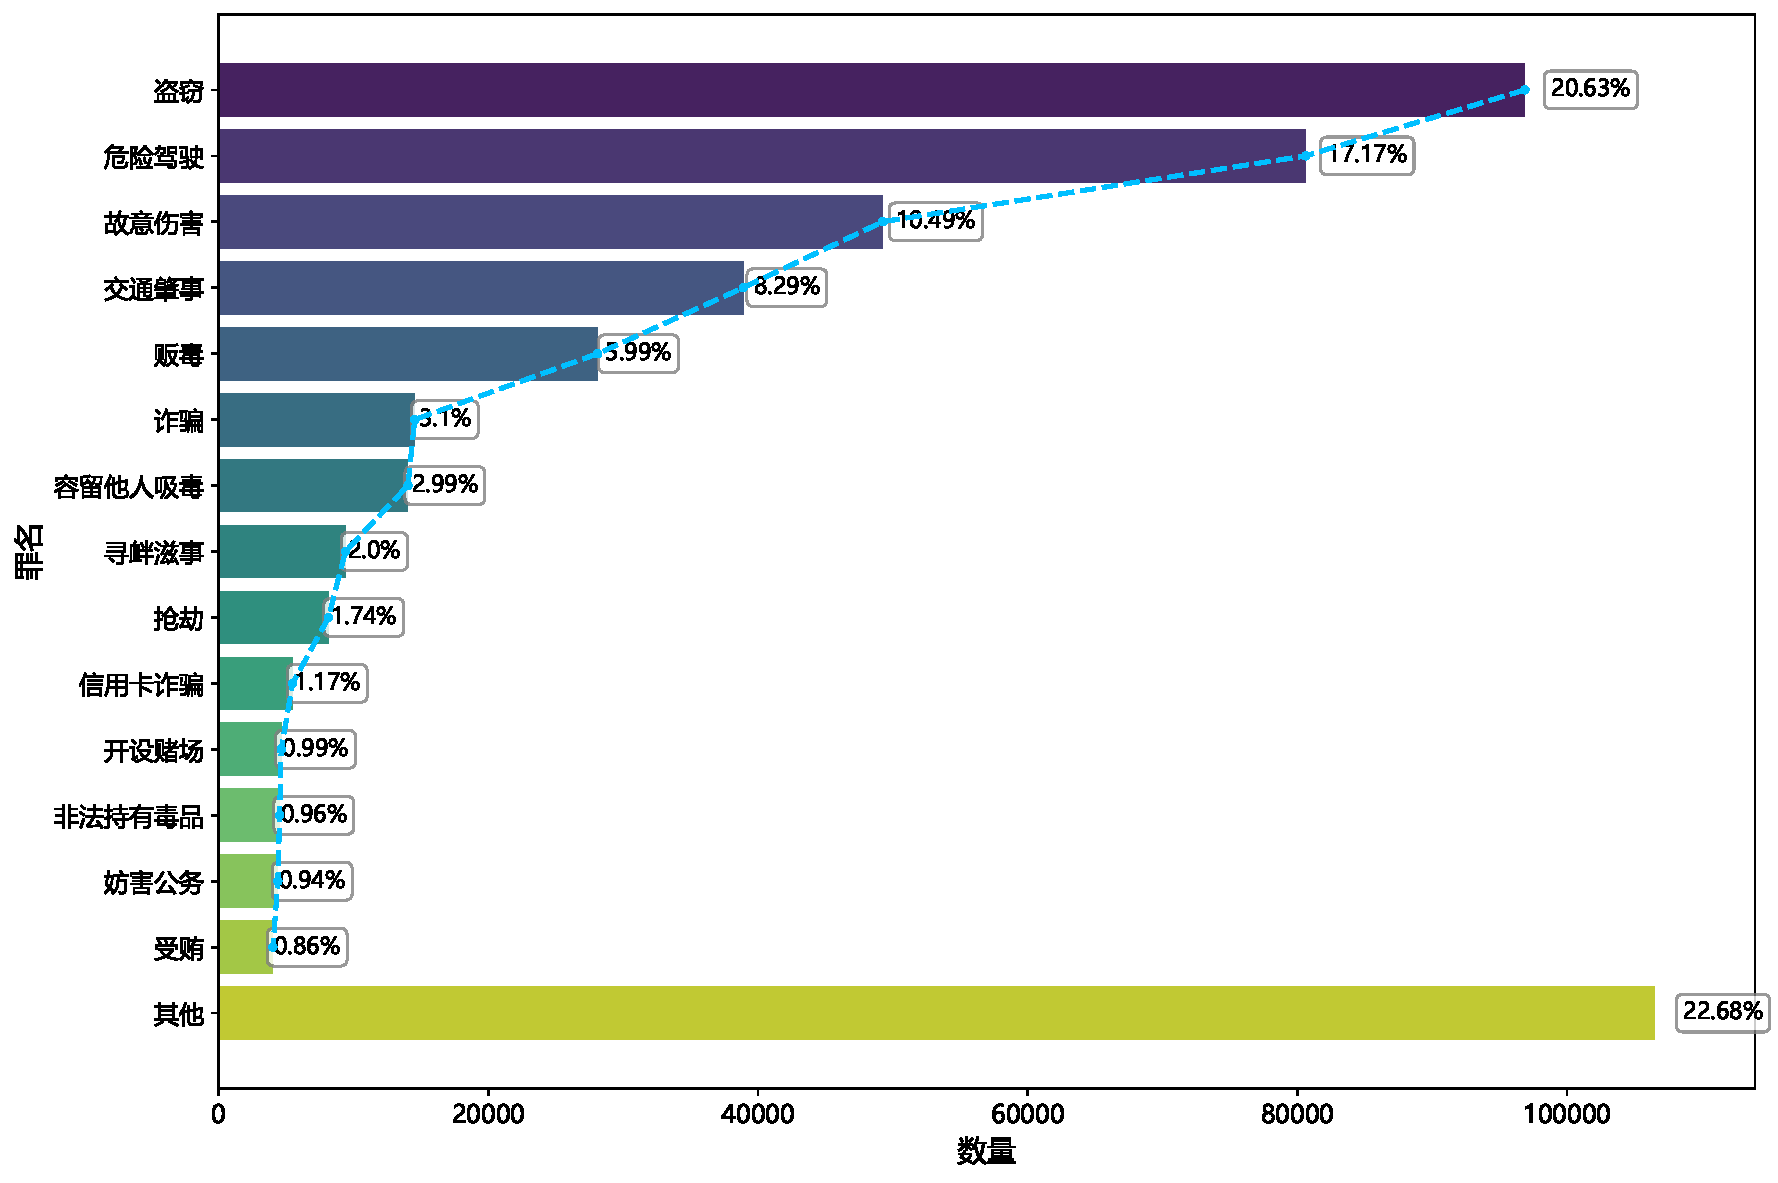
\includegraphics[width=1\linewidth]{fig/accusation_distribution.pdf}
		\caption{测试数据的罪名分布}
		\label{fig:acc_dis}
\end{figure}
如图\ref{fig:art_dis}所示,法条数据分布也呈现长尾趋势。占比最高的10种相关法条占测试数据中0.73\%,而占比最低的100种法条只占2.44\%。
\begin{figure}[H]
    \centering
    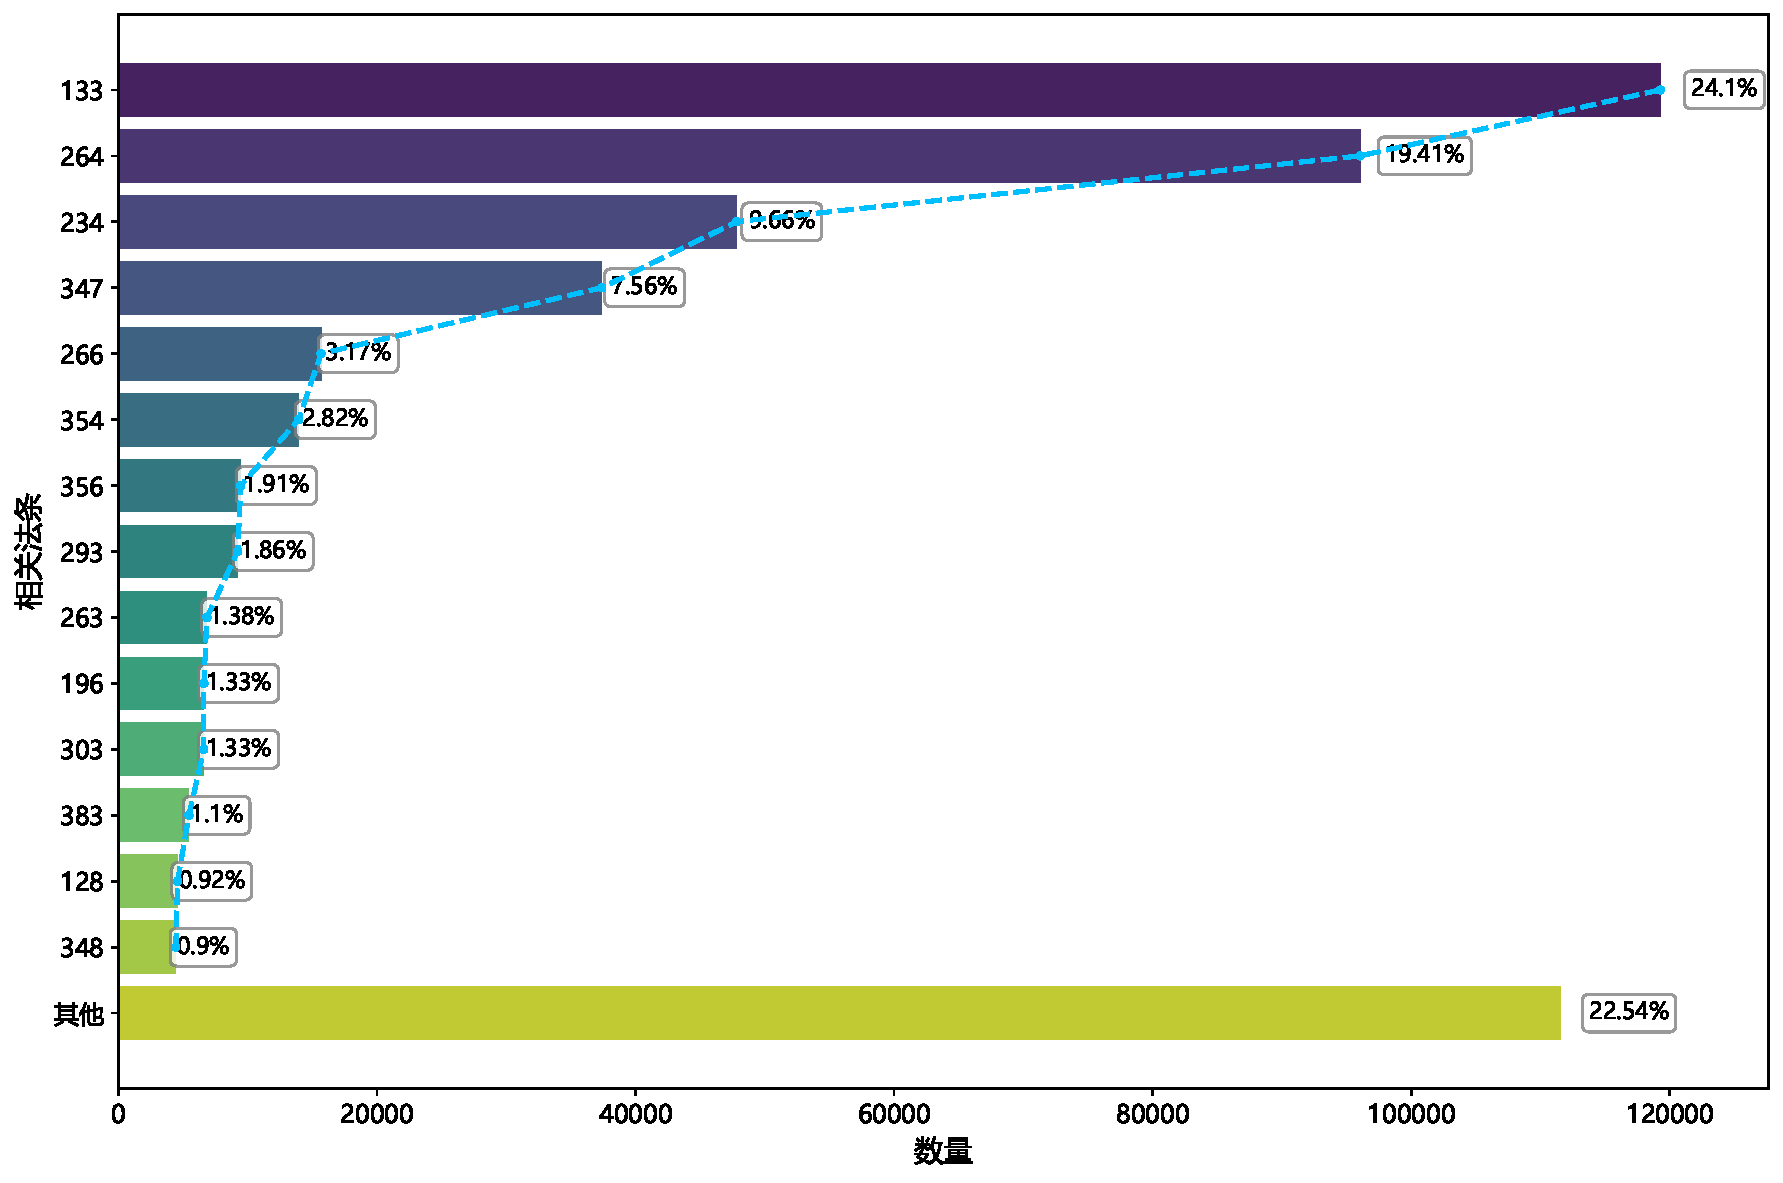
\includegraphics[width=1\linewidth]{fig/article_distribution.pdf}
    \caption{测试数据的法条数据分布}
    \label{fig:art_dis}
\end{figure}
\subsection{\heiti 实验设置}
本研究案例数据库利用CAIL 2018~\cite{xiao2018cail2018largescalelegaldataset}的训练集构造。为了在控制案例数据库规模的同时兼顾检索效率和案例,本研究从训练集中每种罪名最多抽取100条数据,一共构建1676个案例。
法条数据库使用中国刑法作为文本数据。
案例数据库和法条数据库的文本嵌入模型使用BAAI/BGE-m3模型~\cite{chenBGEM3EmbeddingMultiLingual2024};
向量数据库使用milvus~\cite{2022manu,2021milvus},相似度函数使用内积(Inner Product,IP),向量索引方法采用倒排索引(Inverted File,IVF),聚类中心为200个。搜索算法使用暴力搜索(Flat Search,搜索在每个聚类内部时使用相似度函数进行比较。要素提取模型采用qwen-turbo模型
),判决模型使用qwen-plus模型~\cite{qwenQwen25TechnicalReport2025}。

\subsection{\heiti 评价指标}
CAIL 2018法律判决预测中的罪名、刑期预测两项子任务,都属于多标签的多分类问题~\cite{xiao2018cail2018}。
本研究采用精度(Precision , P) 、召回率(Recall , R) 和 F1分数 3项指标来衡量模型的预测效果。
\begin{eqnarray}
		&P=\frac{\sum_{i=1}^{n}TP_{i}}{\sum_{i=1}^{n}TP_{i}+\sum_{i=1}^{n}FP_{i}}
		\\
		&R=\frac{\sum_{i=1}^{n}TP_{i}}{\sum_{i=1}^{n}TP_{i}+\sum_{i=1}^{n}FN_{i}}
		\\
		&F1=\frac{2\times P\times R}{P+R}
\end{eqnarray}
其中,$i$为分类任务中类别的种类;$TP_i$为True Positive,指被正确地划分为类别 $i$ 的样本个数;$FP_i$ 为False Positive,指实际为其他类但被分类器划分为$i$ 类的样本数;$FN_i$ 为False Negative,指实际为 $i$ 类,但是被分类器划分错误的样本数。


\subsection{\heiti 基准模型}
为检验基座LLM的性能和本研究提出的“基于法条约束与类案融合的可解释司法判决预测方法”的有效性,以及与基于域外语料训练的法律大模型能力相比的优劣,本研究进行了CAIL 2018两个子任务罪名和刑期的对比实验,对比本文模型与4种基线模型的效果差异。
基线模型的选取覆盖基于词嵌入的深度学习模型MTL-Fusion~\cite{zhuopeng-etal-2020-multi}模型、中国司法长文本文书预训练模型Lawformer~\cite{xiao2021lawformer},预训练模型BERT~\cite{fan2022multi}以及 司法数据微调与RAG结合LawChatGLM模型~\cite{JSJA202505027}。

\subsection{\heiti 实验结果与分析}


表\ref{tab:performance_comparison}的实验结果清晰地揭示了不同技术路径在法律判决预测任务上的性能差异。从传统模型MTL-Fusion、Lawformer到基于预训练的BERT,再到结合了法律知识增强的LawChatGLM,模型的性能在罪名和刑期预测上呈现出稳步提升的趋势。这证明了更强的语义理解能力和外部知识的引入是提升LJP性能的关键。然而,即便是表现最强的基准模型LawChatGLM,其虽然通过检索法律条文提升了罪名预测的准确性,但在更需酌情裁量的刑期预测上表现仍有较大提升空间(F1分数为0.4691),这表明仅依赖成文法条作为外部知识源尚不足以完全捕捉司法实践的复杂性。

本文提出的方法在所有评价指标上均取得了最优表现,尤其在刑期预测任务上实现了关键突破,F1分数达到0.5525,相较于LawChatGLM提升了8.34\%。这一显著优势的核心原因在于我们创新的“法条约束与类案融合的可解释司法判决预测方法”。该框架不仅通过检索法律条文为罪名判定提供了权威的法律依据,更关键的是,通过引入“相似案例检索”模块,为模型提供了来自真实司法实践的量刑参考。这些相似判例中蕴含的裁判经验和量刑逻辑,有效弥补了成文法条在具体刑期裁量上的模糊性,使得模型的预测更贴近真实的司法裁判思维。实验结果有力地证明,将LLM的推理能力与法律条文的规范性指引、相似案例的实践性参考进行深度融合,是构建高精度、高可靠性智能司法判决系统的有效路径。

\subsection{\heiti 案例研究}
\begin{figure*}[htpb]
    \centering
    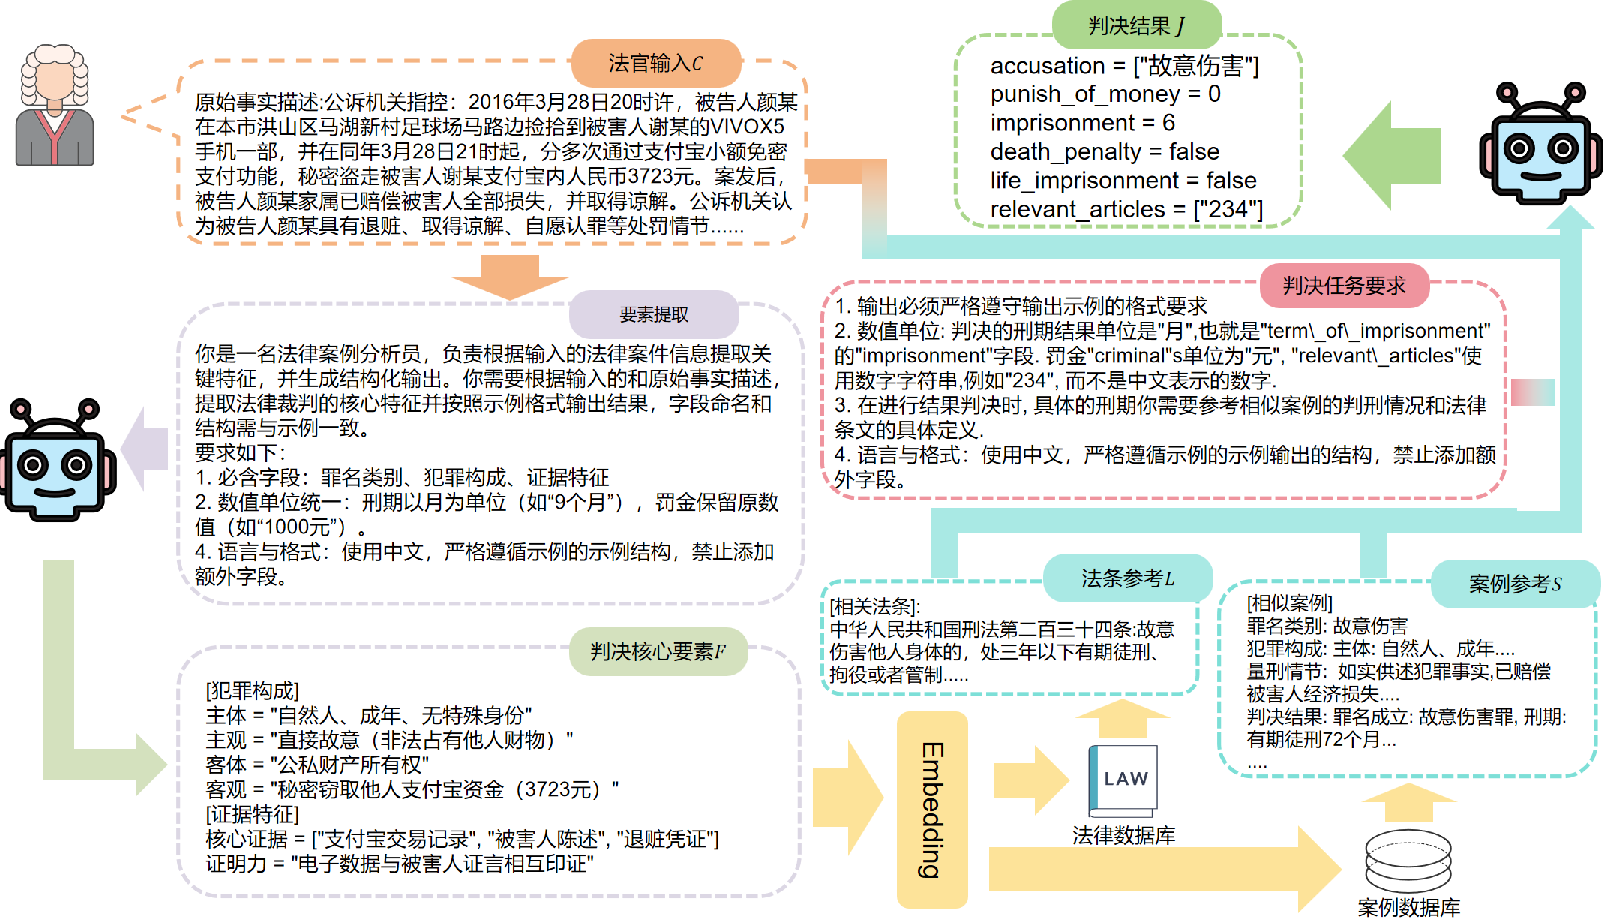
\includegraphics[width=0.8\linewidth]{fig/case.pdf}
    \caption{案例}
    \label{fig:case}
\end{figure*}
本研究提出的方法将以一个具体的盗窃案件为例进行说明。首先,系统接收一段原始的案件事实描述,例如:“公诉机关指控,2016年3月28日20时许,被告人颜某在…盗走被害人谢某支付宝内人民币3723元”。接着,系统利用LLM对该文本进行“判决核心要素提取”,生成结构化的犯罪特征($F$),包括犯罪构成(主体、主观、客体、客观)和核心证据等。随后,进入本方法的核心——双重知识检索阶段。系统会将提取出的核心要素($F$)通过文本嵌入模型BAAI/BGE-m3转换为高维查询向量。该查询向量被用于在两个并行的路径上执行检索:第一条路径中,系统在预先向量化的法律数据库中进行近似最近邻(ANN)搜索,通过计算内积相似度,找出与案件特征最匹配的法律条文($L$),如《中华人民共和国刑法》第二百六十四条;第二条路径中,系统同样利用该查询向量,在向量化的案例数据库中检索相似判例($S$)。此处的案例检索更为精细,它会综合考量罪名、犯罪构成、证据特征等多个维度的相似度,以确保筛选出的历史判例与当前案件具有高度的可比性。最后,将原始案情($C$)、提取的核心要素($F$)、检索到的法律条文($L$)及相似案例($S$)共同作为输入,送入核心的LLM推理引擎,由其进行综合分析与推理,最终生成一个的结构化判决结果($J$):
\\
accusation = ["盗窃罪"]
\\
relevant\_articles = ["264"]
\\
punish\_of\_money = 3723
\\
imprisonment = 7
\\
death\_penalty = false
\\
life\_imprisonment = false



\section{\heiti 结论}
本研究针对当前法律判决预测(LJP)领域中,传统模型因其“黑箱”特性而缺乏可解释性,以及LLM因存在“幻觉”和缺乏专业知识而难以直接应用的双重困境,提出了一种基于法条约束与类案融合的可解释司法判决预测方法。该方法将复杂的判决任务分解为一系列逻辑清晰的子任务:首先通过LLM精准提取判决的核心要素,然后并行地从外部知识库中检索权威的法律条文与高度相似的司法判例,最后再由LLM融合这些多源异构信息,生成最终的判决结果。

实验结果有力地证明了本方法的有效性。我们的方法在罪名和刑期预测任务上的F1分数分别达到了\textbf{0.7743}和\textbf{0.5525},在所有对比模型中取得了最优性能。相较于同样结合了外部知识库的先进基准模型,本方法在罪名预测的F1分数上提升了约\textbf{3.3\%},在对司法实践经验有高度依赖的刑期预测上,性能更是实现了\textbf{17.8\%}的显著提升。这一性能突破的核心贡献在于,本框架通过引入法律条文数据库,为模型的推理提供了坚实的法律依据,有效缓解了内容幻觉问题;更关键的是,通过引入相似案例数据库,模型得以借鉴海量的司法实践经验,从而在对酌情裁量有较高要求的刑期预测上表现卓越。这一结果表明,将LLM的强大语言能力与法律条文的规范性、司法判例的实践性进行深度融合,是提升LJP系统准确性和可靠性的关键。

\subsubsection{参考文献}


\vspace {3mm}
\zihao{5}{
\noindent \textsf{致\quad 谢}\quad \textit{ *致谢内容.* 致谢}}

\vspace {5mm}
\centerline
{\zihao{5}\textsf{参~考~文~献}}
\zihao{5-} \addtolength{\itemsep}{-1em}
\vspace {1.5mm}
\bibliographystyle{gbt7714-numerical}
\bibliography{ref.bib}
\end{multicols}

\begin{multicols}{1}
\noindent {\zihao{5}\bf{附录X}.}

{\zihao{5-}\setlength\parindent{2em}
*\textbf{附录内容}置于此处,字体为小5号宋体。附录内容包括:\textbf{详细的定理证明、公式推导、原始数据}等*}\\\\

\end{multicols}


\begin{multicols}{1}
\begin{biography}[yourphotofilename.jpg]
\noindent
\textbf{First A. Author}\ \ *计算机学报第1作者提供照片电子图片,尺寸为1寸。英文作者介绍内容包括:出生年,学位(或目前学历),职称,主要研究领域(\textbf{与中文作者介绍中的研究方向一致}).*
*字体为小5号Times New Roman*
\end{biography}

\begin{biography}[yourphotofilename.jpg]
\noindent
\textbf{Second B. Author} *英文作者介绍内容包括:出生年,学位(或目前学历),职称,主要研究领域(\textbf{与中文作者介绍中的研究方向一致})。*
*字体为小5号Times New Roman*
\end{biography}
\end{multicols}


\begin{multicols}{1}
\zihao{5}
\noindent \textbf{Background}

\zihao{5-}{
\setlength\parindent{2em}
*论文背景介绍为\textbf{英文},字体为小5号Times New Roman体*

论文后面为400单词左右的英文背景介绍。介绍的内容包括:

本文研究的问题属于哪一个领域的什么问题。该类问题目前国际上解决到什么程度。

本文将问题解决到什么程度。

课题所属的项目。

项目的意义。

本研究群体以往在这个方向上的研究成果。

本文的成果是解决大课题中的哪一部分,如果涉及863$\backslash
$973以及其项目、基金、研究计划,注意这些项目的英文名称应书写正确。}

\end{multicols}
\end{document}
